\documentclass[11pt, a4paper,twocolumn]{jarticle}
\usepackage[dvipdfmx]{graphicx}
\usepackage{listings,jlisting}

\begin{document}
%=============================================================
\section{To understand the current-voltage characteristic of semiconductor diodes($3^{rd} day$)}

\subsection{Purpose}
半導体の電流電圧特性を理解する.
\subsection{Procedure}
Siベースダイオード,LED,ツェナーダイオードの三種類の資料について電流電圧特性を計測する.
この時電流が40mAを超えないように注意する.
またヒステリシス特性を観察するために電圧を上昇させた場合と下降させて行った場合の2通りを2回ずつ測定した.

\subsection{Result}
測定の結果電流電圧の関係をプロットすると以下のようなグラフが得られた.
グラフよりいずれのダイオードもある一定の電圧がかからなければ電流を通さない性質を示した.

LEDについては電流が流れるのと同時に発光し始め,電圧を高くするにつれて光は強くなっていった.またいずれのダイオードも逆方向に電圧をかけても電流は流れなかった.

さらにグラフよりわかるように電圧をあげていった場合も電圧を下げた場合も電流の値は同じ値を取ったためヒステリシス特性は示さなかった.

\begin{figure}[htbp]
 \begin{center}
  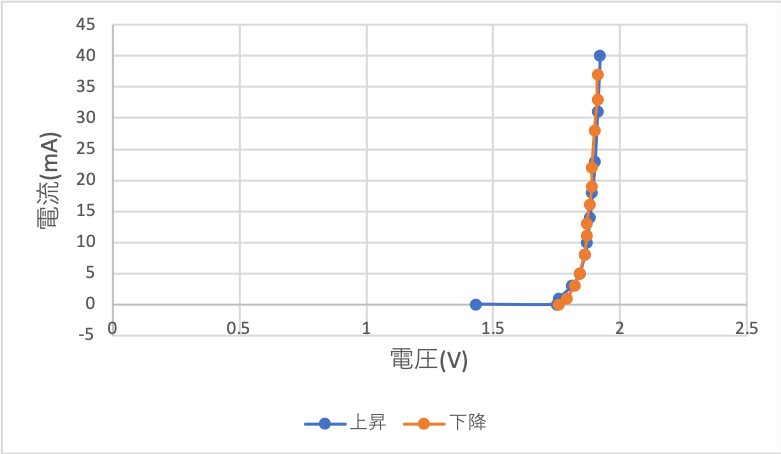
\includegraphics[width=0.8\linewidth]{fig23.png}
 \end{center}
 \caption{LED 1回目}
 \label{fig:23}
\end{figure}

\begin{figure}[htbp]
 \begin{center}
  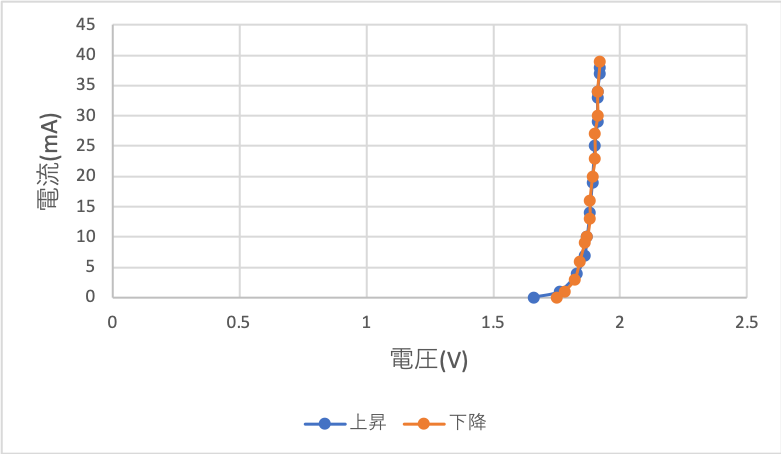
\includegraphics[width=0.8\linewidth]{fig24.png}
 \end{center}
 \caption{LED 2回目}
 \label{fig:24}
\end{figure}

\begin{figure}[htbp]
 \begin{center}
  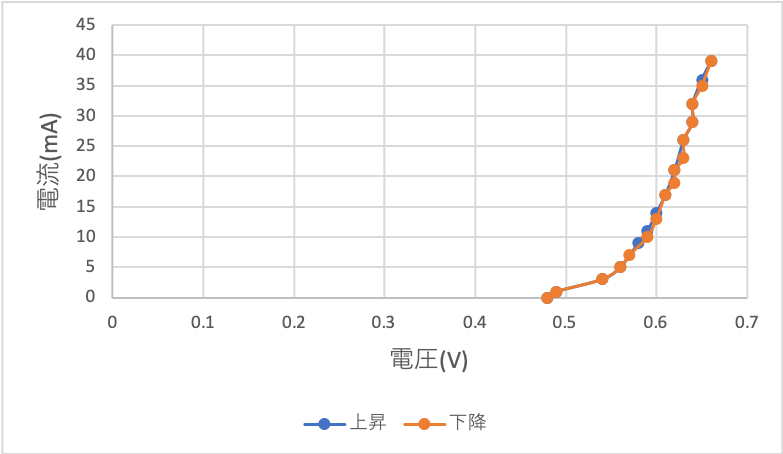
\includegraphics[width=0.8\linewidth]{fig25.png}
 \end{center}
 \caption{Siダイオード 1回目}
 \label{fig:25}
\end{figure}

\begin{figure}[htbp]
 \begin{center}
  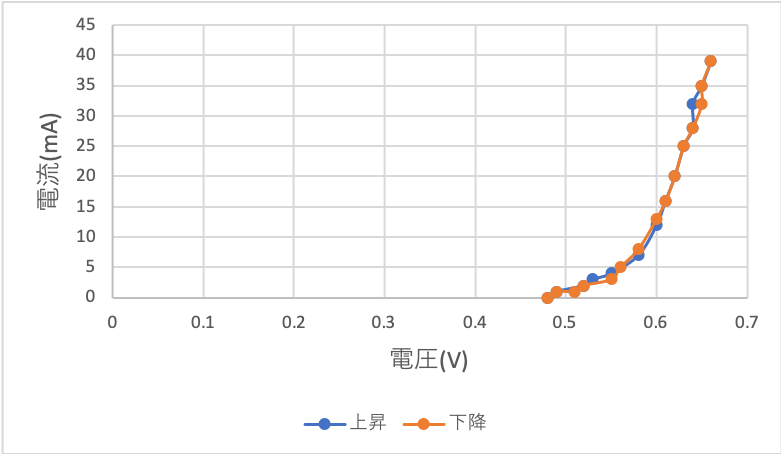
\includegraphics[width=0.8\linewidth]{fig26.png}
 \end{center}
 \caption{Siダイオード 2回目}
 \label{fig:26}
\end{figure}

\newpage

\begin{figure}[htbp]
 \begin{center}
  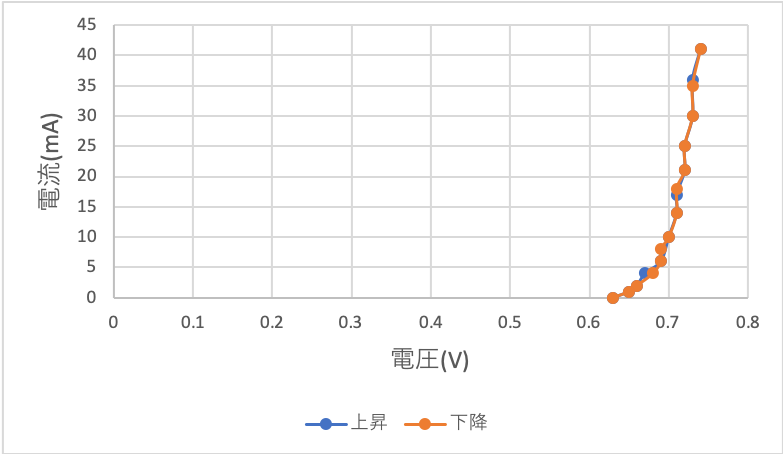
\includegraphics[width=0.8\linewidth]{fig27.png}
 \end{center}
 \caption{ツェナーダイオード 1回目}
 \label{fig:27}
\end{figure}

\begin{figure}[htbp]
 \begin{center}
  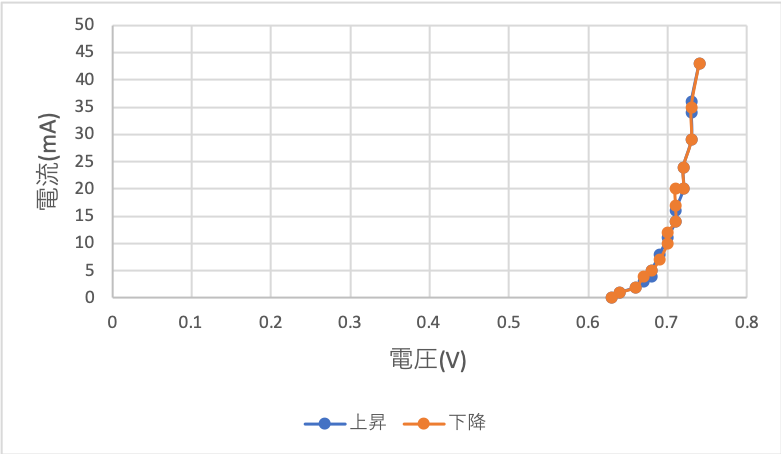
\includegraphics[width=0.8\linewidth]{fig28.png}
 \end{center}
 \caption{ツェナーダイオード 2回目}
 \label{fig:28}
\end{figure}



\subsection{Discussion}
実験結果よりダイオードは順バイアス電圧をかけた際には電流を流すが逆バイアス時には電流は流れない整流作用の特性を持つので電流が逆流して欲しくない回路などに組み込んで応用することができると考えられる.

次にダイオードの順バイアス時にある特定の電圧を超えた際に電流を流し始める特性について考察する.
まずPN接合においては図\ref{fig:36}のようにP領域のキャリアとN領域の電子がそれぞれ接触し消滅する空乏層が生成される.
この空乏層が障壁となるため順バイアスを印加した際にある一定電圧を超えないと電流を流さないのはこの電位障壁が理由だと考えられる.
また逆バイアスをかけた際は空乏層を広げることとなりこの時は電流を流すことはなくなる.これが整流作用の原理だと考えられる.

また逆バイアスをさらに印加していった際の振る舞いについて考察する.
非常に大きな電圧を逆バイアスに印加した際はN型半導体の領域において電子は非常に大きな運動エネルギーを持つことになるがこの運動エネルギーが振動する格子に衝突することで減少し,格子にエネルギーが受け渡されるがこのエネルギーが格子の電子を励起させるのに十分な運動エネルギーを持っていた場合,ぶつかった格子から新たに自由電子とホールのペアが生成される.
またこの反応が再帰的に起こることで急激に電流が流れることが予想される.
今回は実験の時間により逆バイアスの測定ができなかったが図\ref{fig:37}のように電圧電流特性を示すことが予想される.



\begin{figure}[htbp]
 \begin{center}
  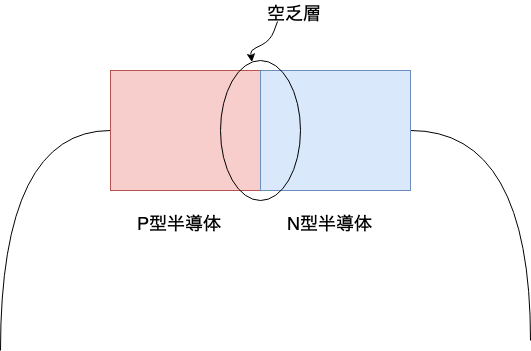
\includegraphics[width=0.8\linewidth]{fig36.png}
 \end{center}
 \caption{PN接合}
 \label{fig:36}
\end{figure}

\begin{figure}[htbp]
 \begin{center}
  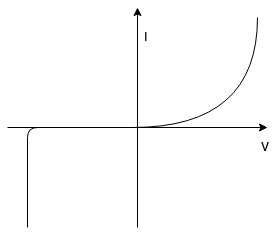
\includegraphics[width=0.8\linewidth]{fig37.png}
 \end{center}
 \caption{電流電圧特性}
 \label{fig:37}
\end{figure}


%=============================================================
\newpage
\end{document}
